\documentclass{article}
\usepackage[utf8]{inputenc}
\usepackage[french]{babel}
\usepackage{graphicx}
\usepackage{listings}
\usepackage{color}
\usepackage{hyperref}
\usepackage{geometry}
\geometry{a4paper, margin=2.5cm}

% Configuration des listings pour le code
\definecolor{codegreen}{rgb}{0,0.6,0}
\definecolor{codegray}{rgb}{0.5,0.5,0.5}
\definecolor{codepurple}{rgb}{0.58,0,0.82}
\definecolor{backcolour}{rgb}{0.95,0.95,0.92}

\lstdefinestyle{mystyle}{
    backgroundcolor=\color{backcolour},   
    commentstyle=\color{codegreen},
    keywordstyle=\color{magenta},
    numberstyle=\tiny\color{codegray},
    stringstyle=\color{codepurple},
    basicstyle=\ttfamily\footnotesize,
    breakatwhitespace=false,         
    breaklines=true,                 
    captionpos=b,                    
    keepspaces=true,                 
    numbers=left,                    
    numbersep=5pt,                  
    showspaces=false,                
    showstringspaces=false,
    showtabs=false,                  
    tabsize=2
}

\lstset{style=mystyle}

\title{\LARGE{\textbf{TP 6 : Intégration Jenkins-Ansible}}}
\author{Votre Nom}
\date{\today}

\begin{document}

\maketitle
\thispagestyle{empty}

\newpage
\tableofcontents
\thispagestyle{empty}
\newpage

\setcounter{page}{1}
\section{Introduction}
Ce rapport présente la réalisation du TP 6 portant sur l'intégration de Jenkins avec Ansible pour automatiser le déploiement d'applications depuis GitHub. Ce projet démontre la mise en place d'un pipeline CI/CD complet qui permet d'extraire du code source depuis un dépôt GitHub et de le déployer automatiquement sur des serveurs cibles à l'aide d'Ansible.

\subsection{Objectifs du TP}
Les principaux objectifs de ce travail pratique sont les suivants :
\begin{itemize}
    \item Configurer Jenkins avec les plugins nécessaires
    \item Créer un pipeline Jenkins qui s'intègre avec GitHub
    \item Automatiser le déploiement d'une application web avec Ansible
    \item Implémenter une solution CI/CD complète
\end{itemize}

\section{Environnement de travail}
\subsection{Configuration système}
\begin{itemize}
    \item Système d'exploitation : Linux 6.12.10-76061203-generic
    \item Shell : /usr/bin/bash
\end{itemize}

\subsection{Outils utilisés}
\begin{itemize}
    \item Jenkins : pour l'orchestration du pipeline CI/CD
    \item Ansible : pour l'automatisation du déploiement
    \item GitHub : pour héberger le code source
    \item Apache : comme serveur web pour l'application déployée
\end{itemize}

\section{Installation et configuration de Jenkins}
\subsection{Installation de Jenkins}
% Étape 1: Installer Jenkins

% Ici, vous ajouterez la capture d'écran de l'installation de Jenkins
% \begin{figure}[h]
%     \centering
%     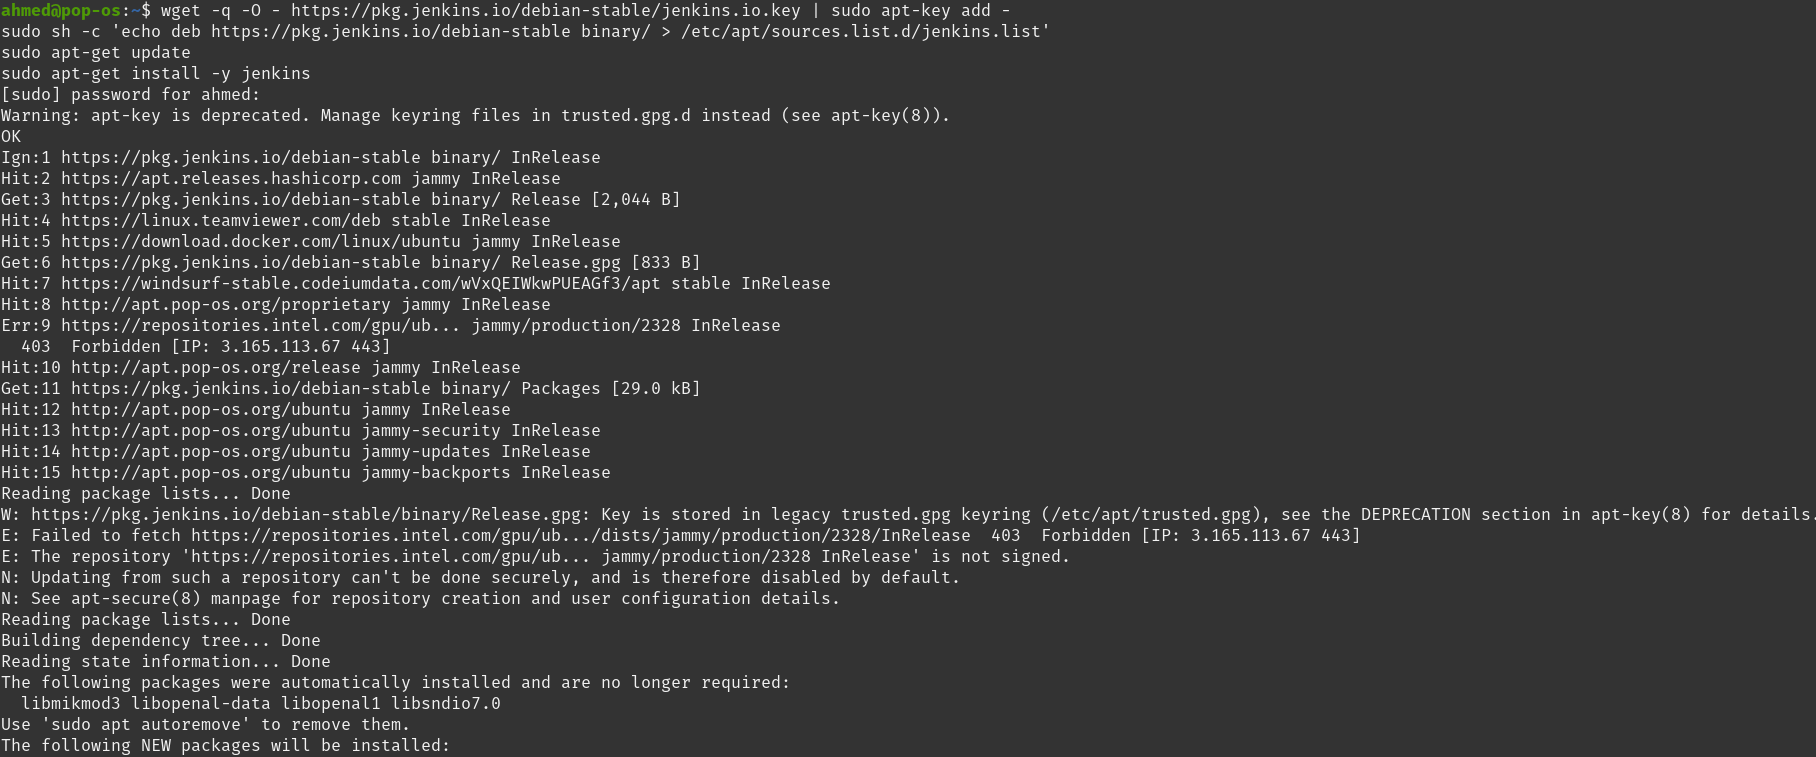
\includegraphics[width=0.8\textwidth]{images/jenkins_installation.png}
%     \caption{Installation de Jenkins}
%     \label{fig:jenkins_installation}
% \end{figure}

J'ai commencé par installer Jenkins en suivant les commandes recommandées :

\begin{lstlisting}[language=bash]
wget -q -O - https://pkg.jenkins.io/debian-stable/jenkins.io.key | sudo apt-key add -
sudo sh -c 'echo deb https://pkg.jenkins.io/debian-stable binary/ > /etc/apt/sources.list.d/jenkins.list'
sudo apt-get update
sudo apt-get install -y jenkins
\end{lstlisting}

Après l'installation, j'ai vérifié que le service Jenkins était bien en cours d'exécution :

\begin{lstlisting}[language=bash]
sudo systemctl status jenkins
\end{lstlisting}

\subsection{Configuration initiale}
Pour la configuration initiale de Jenkins, j'ai récupéré le mot de passe administrateur initial :

\begin{lstlisting}[language=bash]
sudo cat /var/lib/jenkins/secrets/initialAdminPassword
\end{lstlisting}

% Ici, vous ajouterez la capture d'écran de la page de déverrouillage Jenkins
% \begin{figure}[h]
%     \centering
%     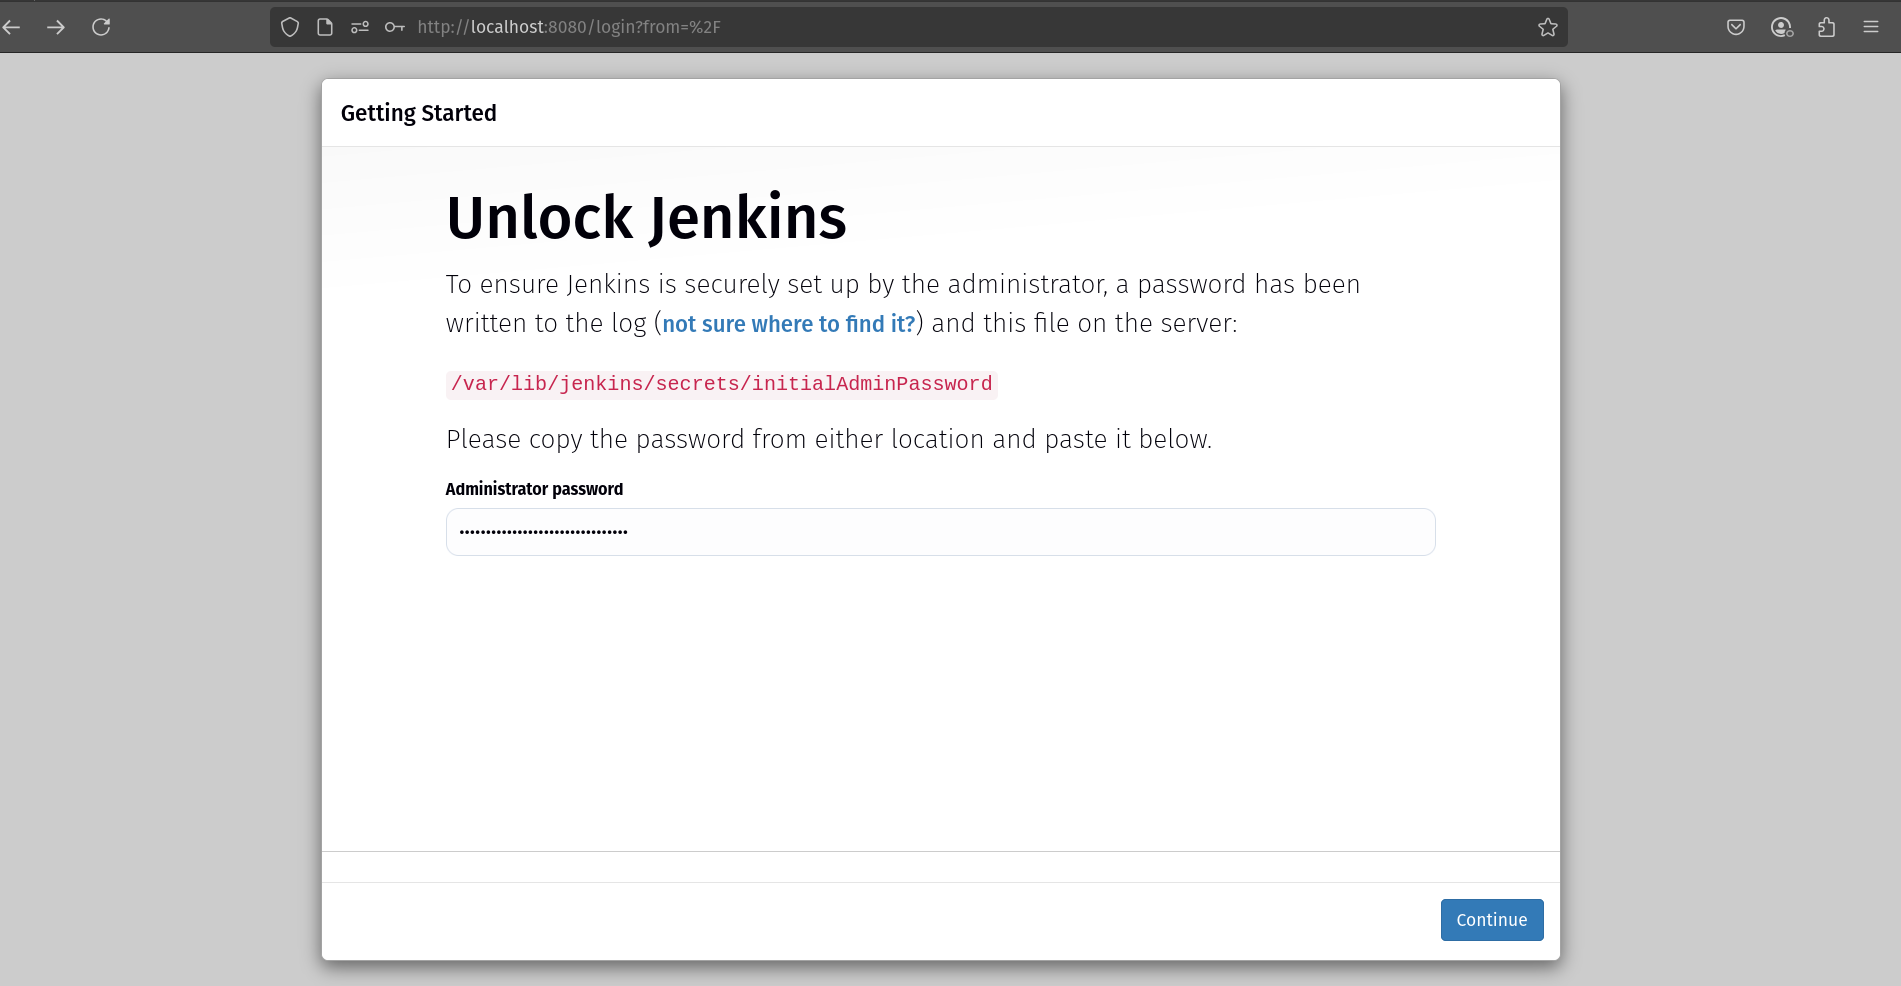
\includegraphics[width=0.8\textwidth]{images/jenkins_unlock.png}
%     \caption{Page de déverrouillage Jenkins}
%     \label{fig:jenkins_unlock}
% \end{figure}

J'ai ensuite suivi l'assistant de configuration pour :
\begin{itemize}
    \item Installer les plugins recommandés
    \item Créer un compte administrateur
    \item Configurer l'URL de Jenkins
\end{itemize}

% Ici, vous ajouterez la capture d'écran de Jenkins après configuration
% \begin{figure}[h]
%     \centering
%     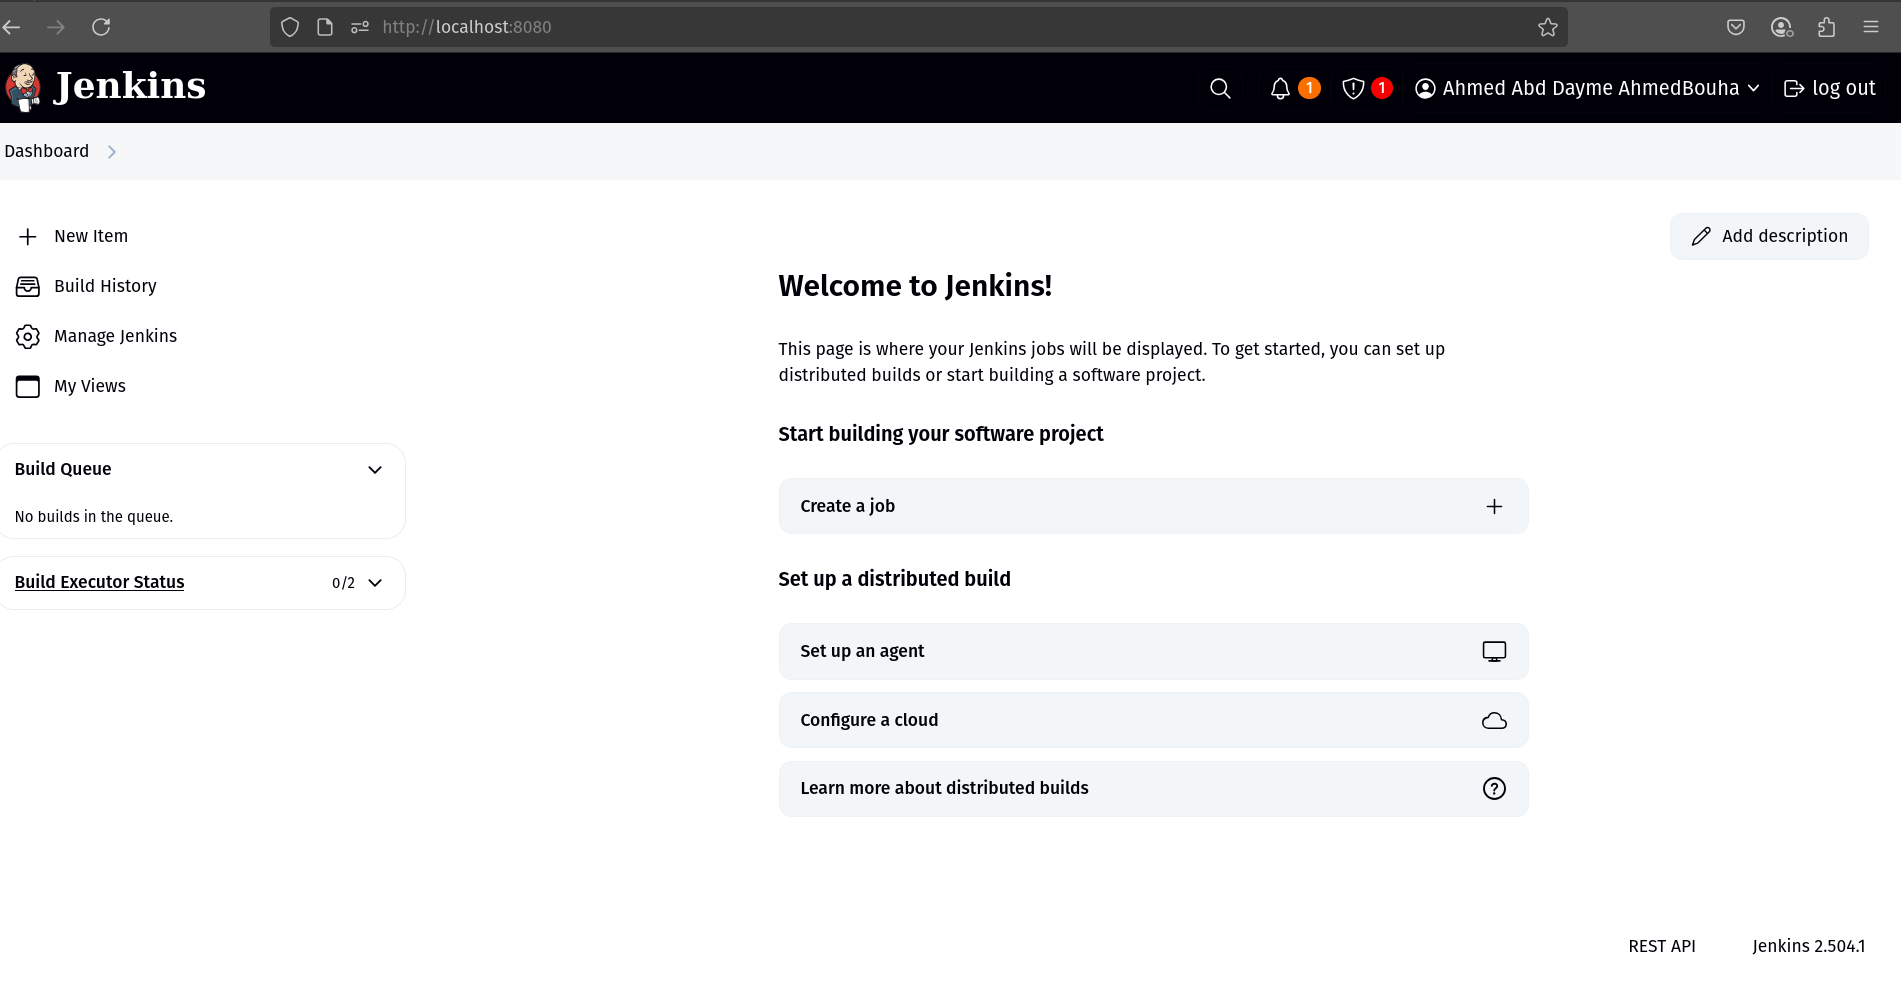
\includegraphics[width=0.8\textwidth]{images/jenkins_dashboard.png}
%     \caption{Dashboard Jenkins après configuration}
%     \label{fig:jenkins_dashboard}
% \end{figure}

\section{Installation des plugins spécifiques}
\subsection{Installation des plugins requis}
Pour ce TP, j'ai installé les plugins suivants depuis l'interface de gestion de plugins de Jenkins (Manage Jenkins > Manage Plugins) :
\begin{itemize}
    \item Git Plugin : pour interagir avec les dépôts Git
    \item GitHub Integration Plugin : pour l'intégration avec GitHub
    \item Ansible Plugin : pour exécuter des playbooks Ansible
\end{itemize}

% Ici, vous ajouterez la capture d'écran de la page des plugins
% \begin{figure}[h]
%     \centering
%     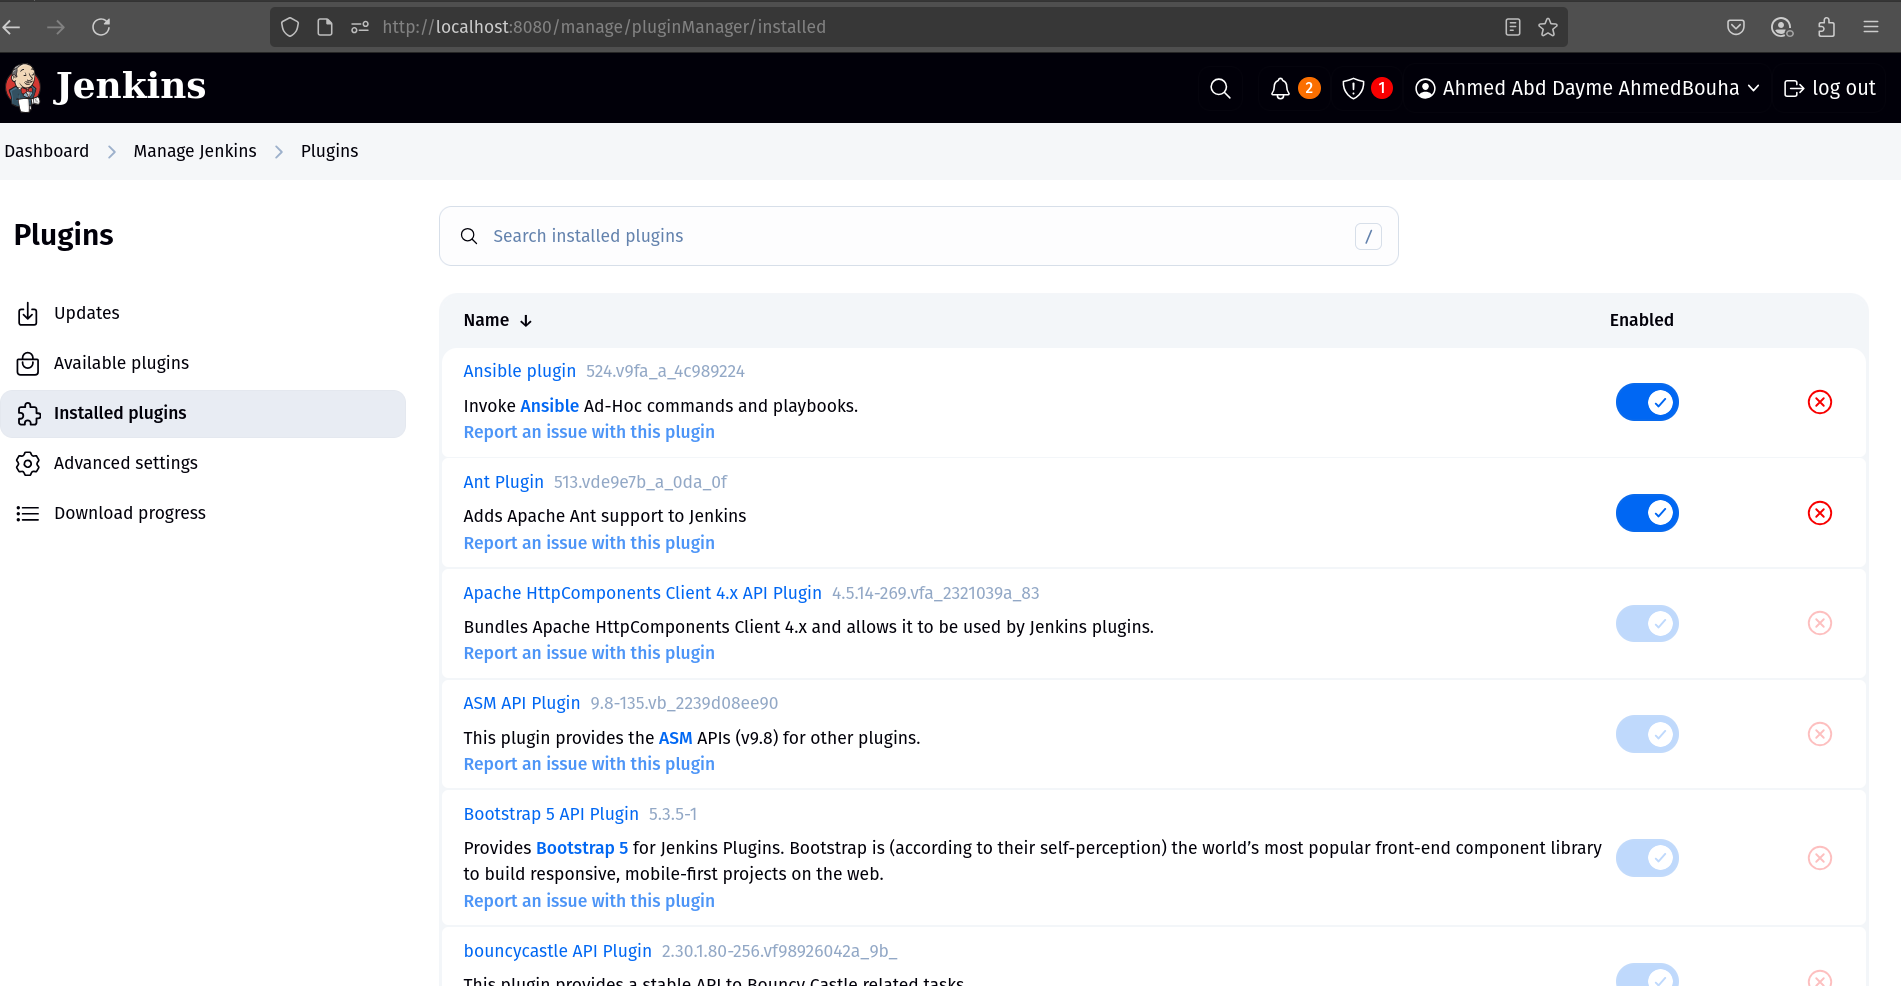
\includegraphics[width=0.8\textwidth]{images/jenkins_plugins.png}
%     \caption{Installation des plugins Jenkins}
%     \label{fig:jenkins_plugins}
% \end{figure}

\section{Préparation du dépôt GitHub}
\subsection{Création et configuration du dépôt}

J'ai créé un dépôt GitHub nommé \texttt{dev\_ansible} pour héberger le code source du projet. Voici les commandes que j'ai utilisées pour initialiser le dépôt :

\begin{lstlisting}[language=bash]
echo "# dev_ansible" >> README.md
git init
git add README.md
git commit -m "first commit"
git branch -M main
git remote add origin git@github.com:ahmedabddayme3752/dev_ansible.git
git push -u origin main
\end{lstlisting}

Ensuite, j'ai ajouté tous les fichiers du projet dans le dépôt :

\begin{lstlisting}[language=bash]
git add .
git commit -m "Add project files"
git push -u origin main
\end{lstlisting}

% Ici, vous ajouterez la capture d'écran du dépôt GitHub
% \begin{figure}[h]
%     \centering
%     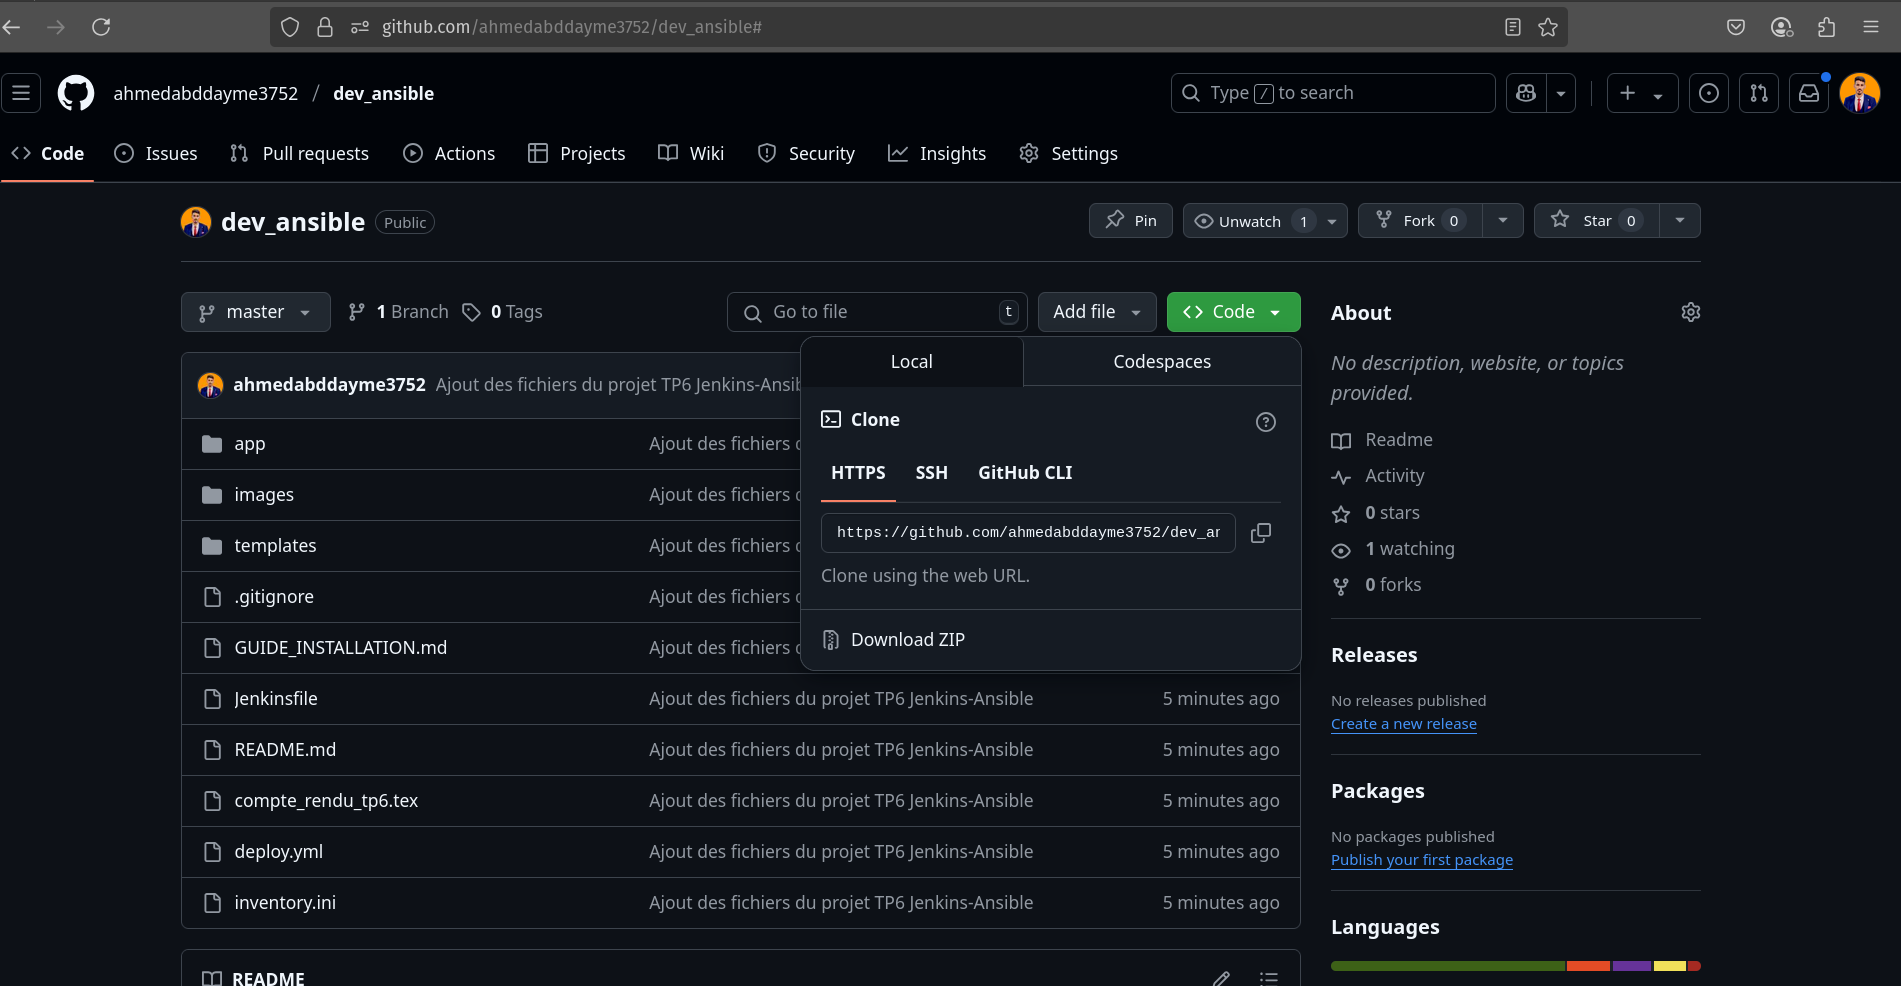
\includegraphics[width=0.8\textwidth]{images/github_repo.png}
%     \caption{Dépôt GitHub avec les fichiers du projet}
%     \label{fig:github_repo}
% \end{figure}

\subsection{Structure du projet}
Le projet contient les fichiers suivants :
\begin{itemize}
    \item \texttt{Jenkinsfile} : Configuration du pipeline CI/CD
    \item \texttt{inventory.ini} : Fichier d'inventaire Ansible définissant les hôtes cibles
    \item \texttt{deploy.yml} : Playbook Ansible pour le déploiement de l'application
    \item \texttt{app/} : Répertoire contenant l'application web à déployer
    \item \texttt{templates/} : Répertoire contenant les templates pour la configuration
\end{itemize}

\section{La suite du compte rendu sera complétée au fur et à mesure de l'avancement du TP}

% Sections à venir :
% - Création et configuration du pipeline Jenkins
% - Configuration d'Ansible
% - Exécution du pipeline
% - Vérification du déploiement
% - Configuration du webhook (Optionnel)
% - Conclusion

\end{document} 